\documentclass[tikz,border=2pt]{standalone}
\usepackage{amsmath,amssymb}
\usepackage{tikz}

\begin{document}
% An event is a subset of the sample space: "the roll is even" is A = {2, 4, 6}.
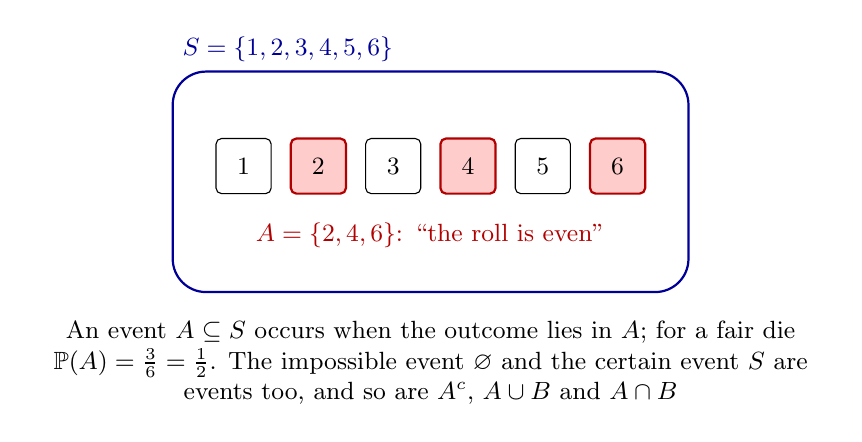
\begin{tikzpicture}[every node/.style={font=\small}]
	\draw[thick, blue!60!black, rounded corners=12pt] (-0.4,-0.4) rectangle (6.15,2.4);
	\node[blue!60!black, anchor=south west] at (-0.4,2.4) {$S=\{1,2,3,4,5,6\}$};
	\foreach \i in {1,3,5} {
		\pgfmathsetmacro{\x}{0.5+(\i-1)*0.95}
		\node[draw, fill=white, rounded corners=2pt, minimum size=7mm] at (\x,1.2) {$\i$};
	}
	\foreach \i in {2,4,6} {
		\pgfmathsetmacro{\x}{0.5+(\i-1)*0.95}
		\node[draw=red!70!black, thick, fill=red!20, rounded corners=2pt, minimum size=7mm] at (\x,1.2) {$\i$};
	}
	\node[red!70!black, anchor=north] at (2.875,0.6) {$A=\{2,4,6\}$: ``the roll is even''};
	\node[anchor=north, align=flush center, text width=10cm] at (2.875,-0.65) {An event $A\subseteq S$ occurs when the outcome lies in $A$; for a fair die $\mathbb{P}(A)=\tfrac36=\tfrac12$. The impossible event $\varnothing$ and the certain event $S$ are events too, and so are $A^c$, $A\cup B$ and $A\cap B$};
\end{tikzpicture}
\end{document}
